\chapter{Introduction}

\section{Overview}


{PARALUTION} is a sparse linear algebra library with focus on exploring fine-grained parallelism, targeting modern processors and accelerators including multi/many-core CPU and GPU platforms. The main goal of this software is to provide a portable library for iterative sparse methods on state of the art hardware. Figure~\ref{paralution-lib-middleware} shows the {PARALUTION} framework as middle-ware between different parallel backends and application specific packages.
 
\begin{figure}[!ht]
\centering
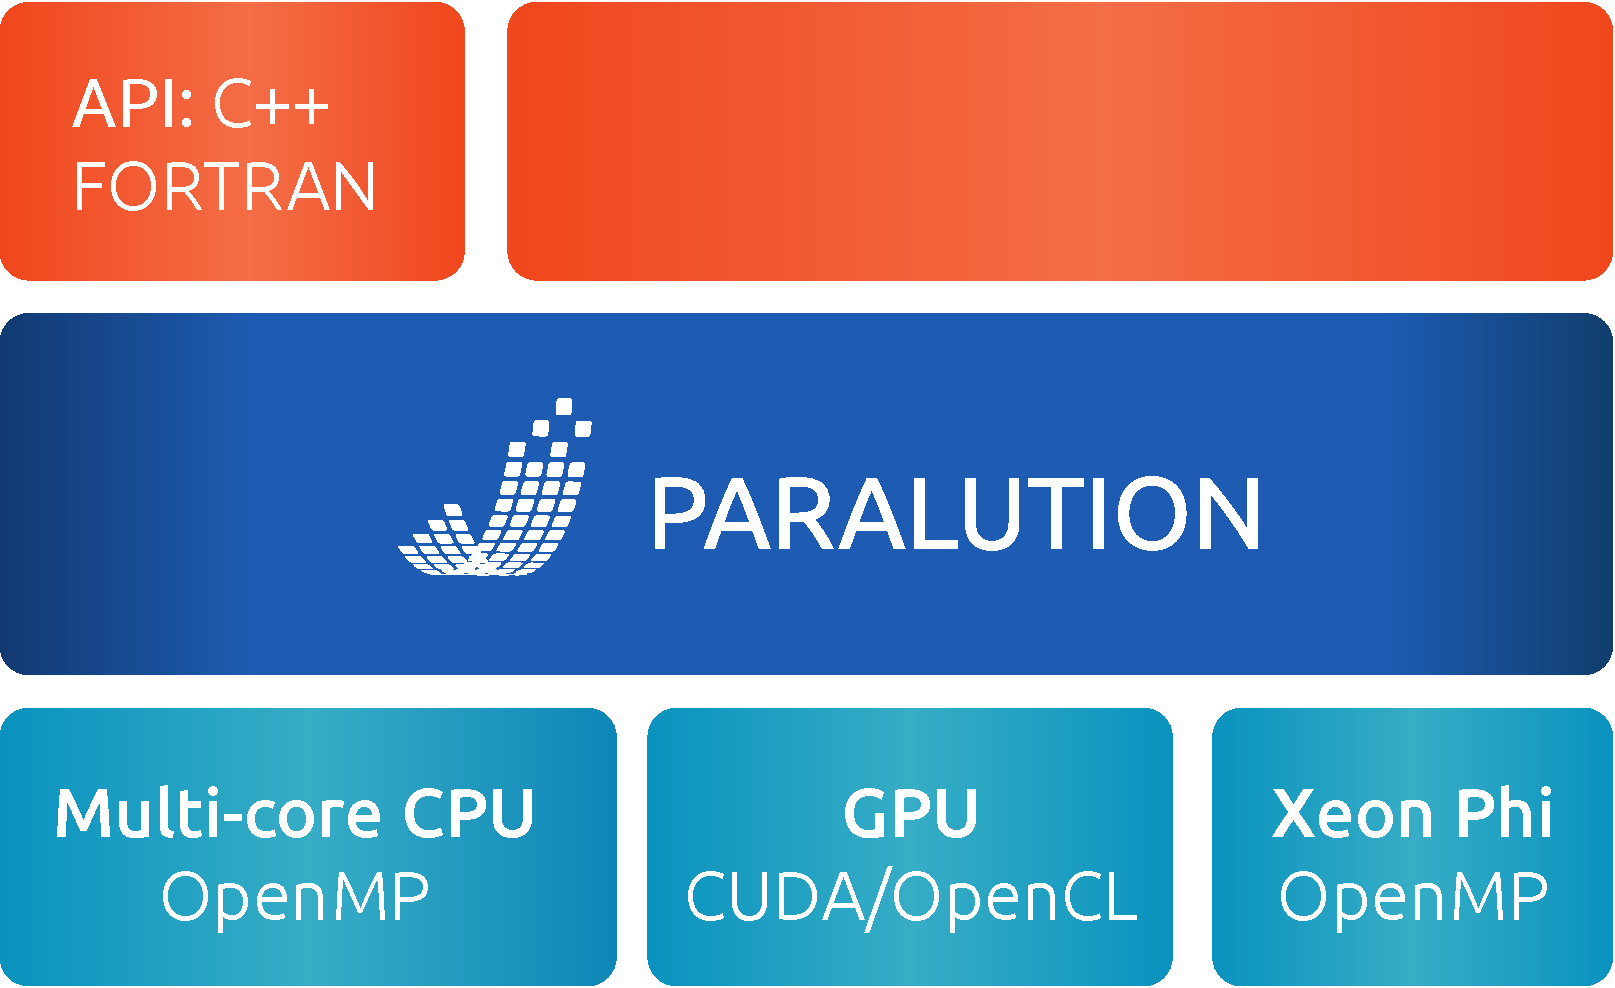
\includegraphics[width=0.5\textwidth]{./fig/paralution-lib.pdf}
\caption{The {PARALUTION} library -- middleware between hardware and problem specific packages.}
\label{paralution-lib-middleware}
\end{figure}


The major features and characteristics of the library are: 

\begin{itemize}

  \item {\bf Various backends}:
\begin{itemize}
  \item Host -- designed for multi-core CPU, based on OpenMP
  \item GPU/CUDA -- designed for NVIDIA GPU
  \item OpenCL -- designed for OpenCL-compatible devices (NVIDIA GPU, AMD GPU, CPU, Intel MIC)
  \item OpenMP(MIC) -- designed for Intel Xeon Phi/MIC
\end{itemize}

 \item {\bf Multi-node/accelerator support} -- the library supports multi-node and multi-accelerator configurations via MPI layer.
 
  \item {\bf Easy to use} -- the syntax and the structure of the library provide fast learning curves. With the help of the examples, anyone can try out the library -- no knowledge in CUDA, OpenCL or OpenMP required.

  \item {\bf No special hardware/library requirements} -- there are no hardware or library requirements to install and run {PARALUTION}. If a GPU device and CUDA, OpenCL, or Intel MKL are available, the library will use them.  

  \item {\bf Most popular operating systems}:
\begin{itemize}
  \item Unix/Linux systems (via cmake/Makefile and gcc/icc)
  \item MacOS (via cmake/Makefile and gcc/icc)
  \item Windows (via Visual Studio)
\end{itemize}

  \item {\bf Various iterative solvers}:
\begin{itemize}
  \item Fixed-Point iteration -- Jacobi, Gauss-Seidel, Symmetric-Gauss Seidel, SOR and SSOR
  \item Krylov subspace methods -- CR, CG, BiCGStab, BiCGStab(l), GMRES, IDR, QMRCGSTAB, Flexible CG/GMRES
  \item Mixed-precision defect-correction scheme
  \item Chebyshev iteration
  \item Multigrid -- geometric and algebraic
\end{itemize}


  \item {\bf Various preconditioners}:
\begin{itemize}
  \item Matrix splitting -- Jacobi, (Multi-colored) Gauss-Seidel, Symmetric Gauss-Seidel, SOR, SSOR
  \item Factorization -- ILU($0$), ILU($p$) (based on levels), ILU($p$,$q$) (power($q$)-pattern method) and Multi-elimination ILU (nested/recursive), ILUT (based on threshold), IC($0$)
  \item Approximate Inverse - Chebyshev matrix-valued polynomial, SPAI, FSAI and TNS
  \item Diagonal-based preconditioner for Saddle-point problems
  \item Block-type of sub-preconditioners/solvers
  \item Additive Schwarz and Restricted Additive Schwarz
  \item Variable type of preconditioners
\end{itemize}

  \item {\bf Generic and robust design} -- {PARALUTION} is based on a generic and robust design, allowing expansion in the direction of new solvers and preconditioners and support for various hardware types. Furthermore, the design of the library allows the use of all solvers as preconditioners in other solvers, for example you can define a CG solver with a Multi-elimination preconditioner, where the last-block is preconditioned with another Chebyshev iteration method which is preconditioned with a multi-colored Symmetric Gauss-Seidel scheme.

  \item {\bf Portable code and results} -- all code based on {PARALUTION} is portable and independent of GPU/CUDA, OpenCL or MKL. The code will compile and run on any supported hardware. All solvers and preconditioners are based on a single source code, which delivers portable results across all supported backends ({\it variations are possible due to different rounding modes on the hardware}). The only difference which you can see for a hardware change is the performance variation.

  \item {\bf Support for several sparse matrix formats} -- Compressed Sparse Row (CSR), Modified Compressed Sparse Row (MCSR), Dense (DENSE), Coordinate (COO), ELL, Diagonal (DIA), Hybrid format of ELL and COO (HYB) formats.

  \item {\bf Plug-ins} -- the library provides a FORTRAN interface.
  
  
\end{itemize}


\section{Purpose of this User Manual}

The purpose of this document is to present the {PARALUTON} library step-by-step. This includes the installation process, internal structure and design, application programming interface (API) and examples. The change log of the software is also listed.

All related documentation (web site information, user manual, white papers, doxygen) follows the Creative Commons Attribution-NonCommercial-NoDerivs 3.0 Unported License \cite{cc}. A copy of the license can be found in the library package.


\section{API Documentation}

The most important library's functions are presented in this document. The library's full API (references) are documented via the automatic documentation system - doxygen \cite{doxygen}. The references are available on the PARALUTION web site.

\section{PARALUTION Versions}

The PARALUTION library is distributed in two different versions.

\begin{figure}[!ht]
  \centering
  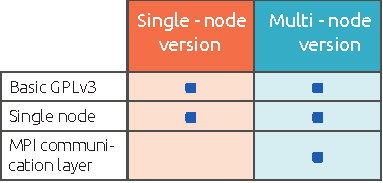
\includegraphics[width=0.65\textwidth]{./fig/ver_new.pdf}
  \caption{The two PARALUTION versions}
  \label{paralution-ver}
\end{figure}

\subsection{Single-node PARALUTION Package}

The single-node PARALUTION version is released under the {GPL} v3 license \cite{gpl}. It contains all single node functionality of the library. This version of the library is free. Please note, that due to the {GPL} v3 license model, any code which uses the library must be released as Open Source and it should have compliance to the {GPL} v3 license.

\subsection{Multi-node PARALUTION Package}

The multi-node PARALUTION version is also released under the {GPL} v3 license \cite{gpl}. The multi node version combines all single node and multi node functionality of the library. This version of the library is free. Please note, that due to the {GPL} v3 license model, any code which uses the library must be released as Open Source and it should have compliance to the {GPL} v3 license.

\section{Version Nomenclature}

Please note the following compatibility policy with respect to the versioning. The version number {x.y.z} represents: x is the major (increases when modifications in the library have been made and/or a new API has been introduced), y is the minor (increases when new functionality (algorithms, schemes, etc) has been added, possibly small/no modification of the API) and z is the revision (increases due to bugfixing or performance improvement). The alpha and beta versions are denoted with {\it a} and {\it b}, typically these are pre-released versions. 

As mentioned above there are two versions of PARALUTION, each release has the same version numbering plus an additional suffix for each type. They are abbreviated with "S" for the single-node version and with "M" for the multi-node version.

\section{Features Nomenclature}

The functions described in this user manual are based on the following nomenclature:
\begin{itemize}
  \item \emph{ValueType} -- type of values can be double (D), float (F), integer (I), and complex (double and float). The particular bit representation (8, 16, 32, 64bit) depends on your compiler and operating system.
  \item \emph{Computation} -- on which backend the computation can be performed, the abbreviation follows: Host backend with OpenMP
(H); CUDA backend (C); OpenCL backend (O); Xeon Phi backend with OpenMP (X). 
  \item \emph{Available} -- in which version this functionality is available: Single-node version (S); Multi-node version (M).
\end{itemize}

The following example states that the function has double, float, integer and complex support; it can be performed on Host backend with OpenMP, CUDA backend, OpenCL backend, Xeon Phi backend with OpenMP; and it is available in both versions of the library.

\begin{table}[H]
\begin{tabular}{l|l|l}
\multicolumn{1}{c|}{ValueType} & Computation & Available \\ \hline
D,F,I,C                        & H,C,O,X     & S,M    
\end{tabular}
\end{table}

Solvers and preconditioners split the computation into a \emph{Building phase} and \emph{Solving phase} which can have different computation backend performance. In the following example the solver/preconditioner support double, float and complex; the building phase can be performed only on the Host with OpenMP or on CUDA; the solving phase can be performed on all other backends; it is available only in the multi-node version of the library.

\begin{table}[H]
\begin{tabular}{l|l|l|l}
\multicolumn{1}{c|}{ValueType} & Building phase & Solving phase & Available \\ \hline
D,F,C                          & H,C            & H,C,O,X       & M
\end{tabular}
\end{table}

\section{Cite}

If you want to cite the PARALUTION library, you can do it by citing our web site. Please specify the version of the software or/and date of accessing our web page:
\begin{lstlisting}
@misc{paralution,
author="{D. Lukarski, N. Trost}",
title="{PARALUTION vX.Y.Z}",
year="20XX",
note = {\url{http://www.paralution.com/}}
}
\end{lstlisting}

\section{Website}

The official web site of the library is
\\
http://www.paralution.com
